\documentclass[writeup.tex]{subfiles}
\begin{document}


\section{Part 1: A Most Curious Business Card}
	Alright, so the business card that dear ol' Santa dropped is the one seen in \autoref{img.santas_business_card}. It shows that Mr. Claus is using both Twitter and Instagram. 

	\begin{figure}[H]
		\centering
		
\includegraphics[scale=.50]{images/santawclaus_shadow}
		\caption{Santa's business card}
		\label{img.santas_business_card}
	\end{figure}
		
		
	\subsection{What is the secret message in Santa's tweets?}
		First things first, looking at Santa's tweets, well, makes me think of a madman. More specifically Wanev\footnote{The old coordinator of the Residence For The Magically Deviant, who gave memoes of "nonsense" when talked to. Seriously though, \textit{always keep the pentaloons.}}. However, that illusion was quickly dispelled, and I realised that I'd probably have to fetch all the tweets to see what was up with them.\\
		\\
		I'll admit though, that I was a little bit on the lazy side when I solved this challenge. I didn't have a script to fetch the tweets and there weren't that many that I bothered writing one, so here's how I did.\\
		\\		
		 So what I did was to load all the tweets by Santa in my browser. This involved scrolling down for a little bit. Once there were no more tweets to load, I pressed \lstinline!CTRL+A! to select all text on the page and then I copied it. \\
		\\
		Next step was to paste it into a text editor, from here it's clear that the content of each tweet is the same length, this can be seen in \autoref{fig.tweets_unfiltered}. 
	
		\begin{figure}[H]
			\centering
			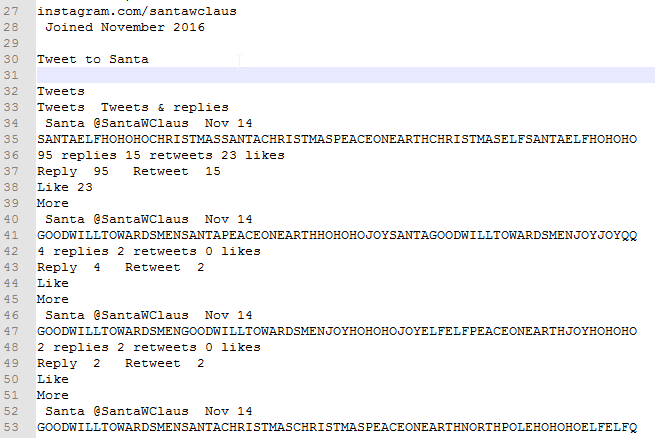
\includegraphics[width=.5\linewidth]{screenshots/tweets_unfiltered}
			\caption{Santa's tweets, unfiltered.}
			\label{fig.tweets_unfiltered}
		\end{figure}

		As it turns out, the content of the tweets are $75$ characters each, this makes removing all the other junk a small task. To remove all the unwanted lines I used a little bit of regex-magic. \\
		\\
		Firstly replacing all lines that were not exactly 75 characters long with an empty string (\autoref{fig.tweets_filtered_p1}) and secondly replacing all multiples of newlines with a single newline (\autoref{fig.tweets_filtered_p2}).

		\begin{figure}[H]
			\centering
			\begin{minipage}{.5\textwidth}
				\centering
				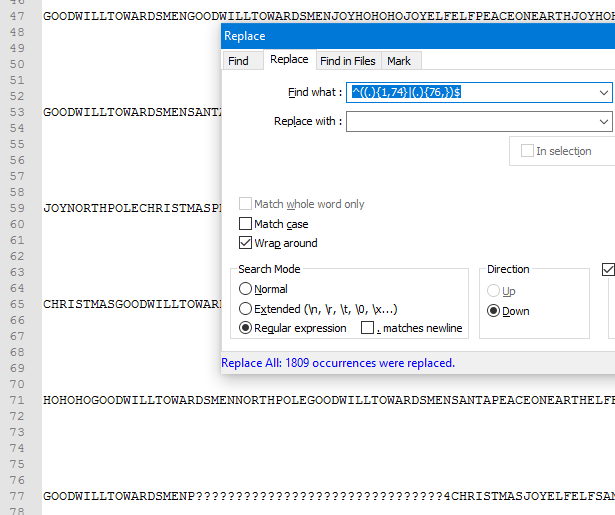
\includegraphics[width=0.9\linewidth]{screenshots/tweets_filtered_p1}
				\caption{Santa's tweets, 1st pass.}
				\label{fig.tweets_filtered_p1}
			\end{minipage}%
			\begin{minipage}{.5\textwidth}
				\centering
				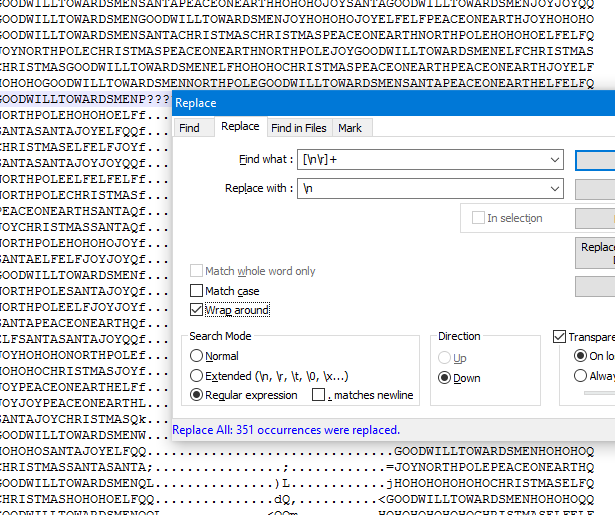
\includegraphics[width=0.9\linewidth]{screenshots/tweets_filtered_p2}
				\caption{Santa's tweets, 2nd pass.}
				\label{fig.tweets_filtered_p2}
			\end{minipage}
		\end{figure}
		
		After doing this, some text is revealed, it is possible to see the outline of a B in \autoref{fig.tweets_filtered_p2}, however, zooming all the way out and rotating the text reveals the secret that is hidden in dear ol' Santa's tweets.
		
		\begin{figure}[H]
			\centering
			
\includegraphics[width=\linewidth]{screenshots/tweets_bug_bounty}
			\caption{Santa's tweets, revelation.}
			\label{fig.tweets_revelation}
		\end{figure}

	\subsection{What is inside the ZIP file distributed by Santa's team?}
		Uh, what? What ZIP file? ... I spend more time on tracking down the ZIP file, than I care to admit. Anyway, here is a run-down of the process of finding said ZIP file.\\
		\\
		I guess we're done with Twitter, so visit Instagram and see 3 beautiful images, two of which I discard more or less at a glance, however \autoref{fig.instagram_messy} looks promising.
		\begin{figure}[H]
			\centering
			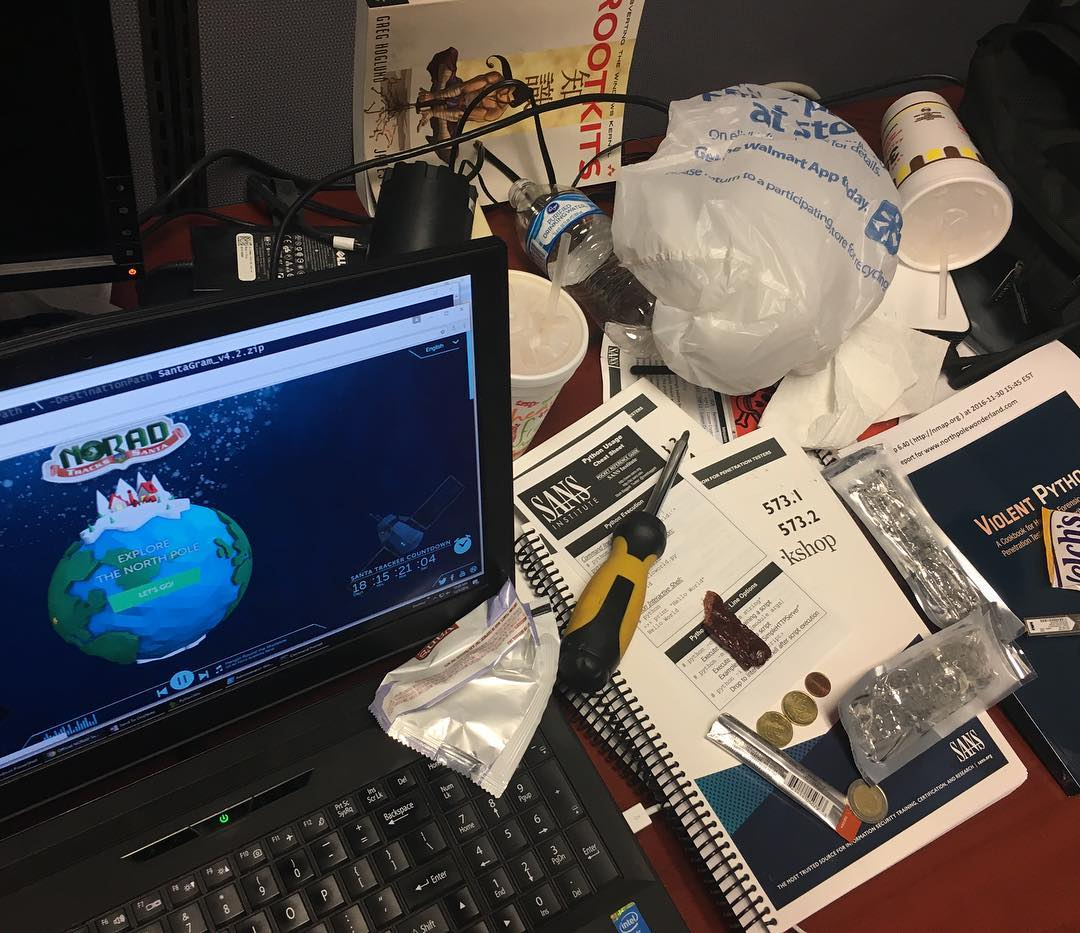
\includegraphics[width=.8\linewidth]{images/instagram}
			\caption{Hermey's messy desk. Unlike mine, which is sparkling...}
			\label{fig.instagram_messy}
		\end{figure}
		
		It doesn't take long to notice the filename of the ZIP file, this can be seen in \autoref{fig.instagram_filename}. But uhm, where exactly should I find this file..? And this is the part that took me longer than I care to admit..\\
		
		\begin{figure}[H]
			\centering
			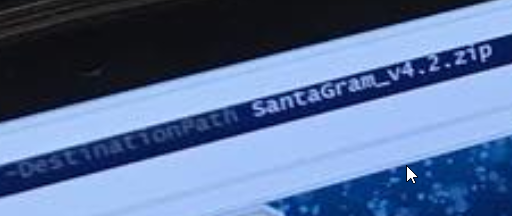
\includegraphics[scale=0.8]{screenshots/instagram_zip_filename}
			\caption{The filename of the ZIP file.}
			\label{fig.instagram_filename}
		\end{figure}
		
		What else is on that picture, a reference to a SANS course, Violent Python, an NMAP report\footnote{... Yup, I completely missed that.}, some half eaten beef jerky(?), a screw driver, various coins, a book called Rootkits, etc. etc. etc., so I think to myself, alright, maybe that's what there is to find in this picture. Time to look at the other two. Now after looking at the other pictures for a while, going back to Twitter to see if I missed something, then going back to Instagram\footnote{I even created an Instagram account, just to make sure that something wasn't hidden behind a login.}, because surely, I must've missed something.\\
		\\
		Aaand suddenly, lightning strikes and I spot the thing that I've completely missed/ignored the whole time. Yup, it's a website, and it can be seen in \autoref{fig.instagram_website}.

		\begin{figure}[H]
			\centering
			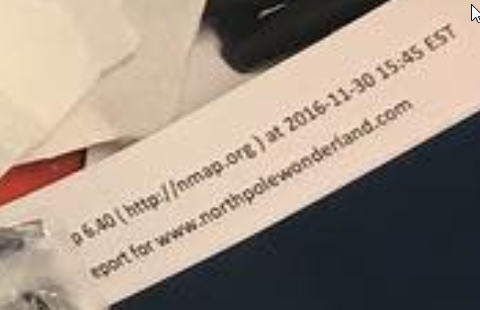
\includegraphics[scale=1]{screenshots/instagram_nmap_report}
			\caption{The filename of the ZIP file.}
			\label{fig.instagram_website}
		\end{figure}
		
		Time to put the two pieces of information together and visit \url{www.northpolewonderland.com/SantaGram_v4.2.zip} and see what's inside the cursed ZIP archive. As seen in \autoref{fig.zipfile_contents} there resides an APK file.\\
		
		\begin{figure}[H]
			\centering
			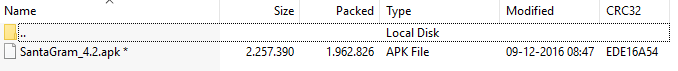
\includegraphics[width=\linewidth]{screenshots/santagram_zip_contents}
			\caption{Contents of ZIP file.}
			\label{fig.zipfile_contents}
		\end{figure}
		
\end{document}